\documentclass[11pt,tikz,border=0pt]{standalone}
\usepackage[T1]{fontenc}
\usepackage{newpxtext,amsmath,newpxmath,graphicx}
\begin{document}
\begin{tikzpicture}[x=1mm,y=1mm,every node/.style={font=\normalsize}]
\path[use as bounding box] (0,0) rectangle (125,50);
\node[anchor=south west,inner sep=0] at (0,0) {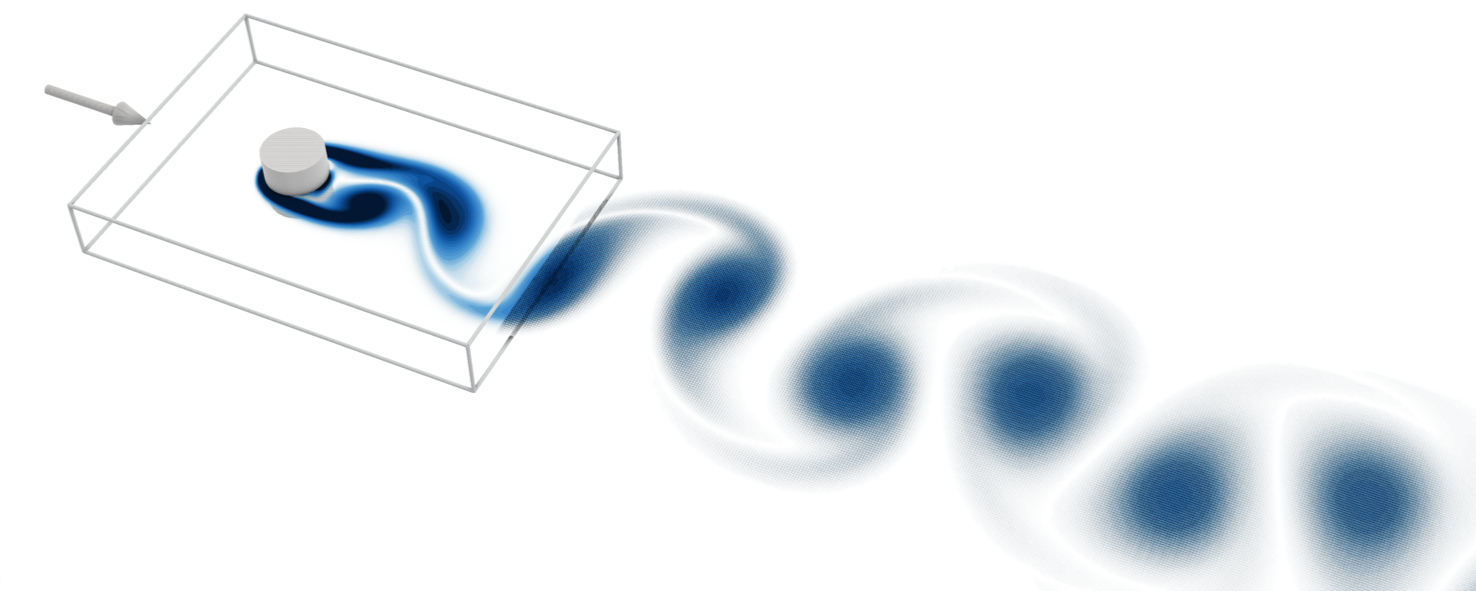
\includegraphics[width=125mm]{cylinder_wake_t86_raw.png}};
\node[anchor=south,inner sep=.8mm] at (8.44,41.60) {$\mathbf{U}_\infty$};
\definecolor{bar0}{rgb}{0.7882,0.9020,0.9922}
\fill[bar0] (97.000,45.0) rectangle ++(1.562,2.0);
\definecolor{bar1}{rgb}{0.6983,0.8622,0.9942}
\fill[bar1] (98.562,45.0) rectangle ++(1.562,2.0);
\definecolor{bar2}{rgb}{0.6084,0.8225,0.9963}
\fill[bar2] (100.125,45.0) rectangle ++(1.562,2.0);
\definecolor{bar3}{rgb}{0.5184,0.7827,0.9984}
\fill[bar3] (101.688,45.0) rectangle ++(1.562,2.0);
\definecolor{bar4}{rgb}{0.4353,0.7407,0.9953}
\fill[bar4] (103.250,45.0) rectangle ++(1.562,2.0);
\definecolor{bar5}{rgb}{0.3725,0.6915,0.9765}
\fill[bar5] (104.812,45.0) rectangle ++(1.562,2.0);
\definecolor{bar6}{rgb}{0.3098,0.6424,0.9576}
\fill[bar6] (106.375,45.0) rectangle ++(1.562,2.0);
\definecolor{bar7}{rgb}{0.2471,0.5932,0.9388}
\fill[bar7] (107.938,45.0) rectangle ++(1.562,2.0);
\definecolor{bar8}{rgb}{0.1937,0.5388,0.9012}
\fill[bar8] (109.500,45.0) rectangle ++(1.562,2.0);
\definecolor{bar9}{rgb}{0.1498,0.4792,0.8447}
\fill[bar9] (111.062,45.0) rectangle ++(1.562,2.0);
\definecolor{bar10}{rgb}{0.1059,0.4196,0.7882}
\fill[bar10] (112.625,45.0) rectangle ++(1.562,2.0);
\definecolor{bar11}{rgb}{0.0620,0.3600,0.7318}
\fill[bar11] (114.188,45.0) rectangle ++(1.562,2.0);
\definecolor{bar12}{rgb}{0.0431,0.2965,0.6212}
\fill[bar12] (115.750,45.0) rectangle ++(1.562,2.0);
\definecolor{bar13}{rgb}{0.0327,0.2316,0.4925}
\fill[bar13] (117.312,45.0) rectangle ++(1.562,2.0);
\definecolor{bar14}{rgb}{0.0222,0.1668,0.3639}
\fill[bar14] (118.875,45.0) rectangle ++(1.562,2.0);
\definecolor{bar15}{rgb}{0.0118,0.1020,0.2353}
\fill[bar15] (120.438,45.0) rectangle ++(1.562,2.0);
\draw[line width=.6pt] (97.0,45.0) rectangle ++(25.0,2.0);
\draw[line width=.6pt] (97.0,45.0) -- ++(0,-0.8);
\node[anchor=north,inner sep=.3mm] at (97.0,44.2) {$0$};
\draw[line width=.6pt] (109.5,45.0) -- ++(0,-0.8);
\node[anchor=north,inner sep=.3mm] at (109.5,44.2) {$1.5$};
\draw[line width=.6pt] (122.0,45.0) -- ++(0,-0.8);
\node[anchor=north,inner sep=.3mm] at (122.0,44.2) {$3$};
\node[anchor=north,inner sep=.3mm] at (109.5,39.8) {$|\boldsymbol{\omega}|\,D/U_\infty$};
\end{tikzpicture}
\end{document}
